\documentclass[border={-3 4 -4 -5}]{standalone}

\usepackage{physics}
\newcommand{\mcD}{\mathcal{D}}

\usepackage{graphicx}
\graphicspath{{../}}

\usepackage{tikz}

\begin{document}
\small
\begin{tikzpicture}
\begin{scope}[shift={(0,-6)}]p
% Mean level spacing ratio{
\node (listdensityplotr) at (0,0.05) {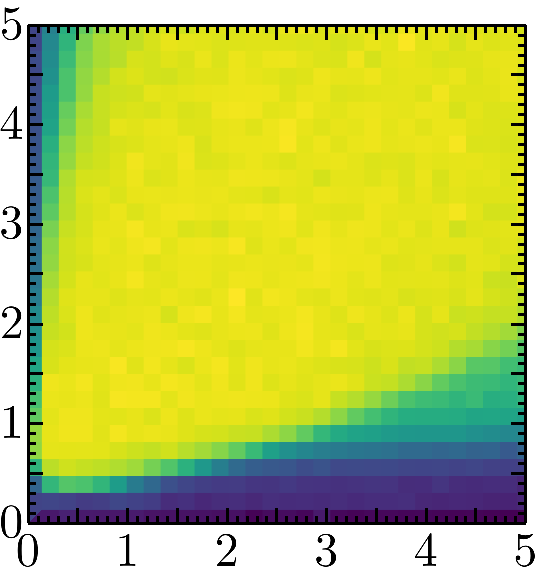
\includegraphics[width=0.325\textwidth]{mean_level_spacing_ratio_xxz_L_18_spinsUp_7_d_9_omega_0.pdf}};
\node[rotate=90] () at ([xshift=-3pt,yshift=0pt]listdensityplotr.west) [] {$J_{xy}/J_z$};
\node (barlegend) at (listdensityplotr.north) [anchor=south, inner sep=-7pt]  {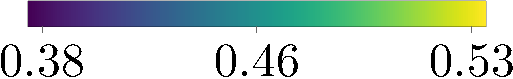
\includegraphics[width=0.27\textwidth]{mean_level_spacing_ratio_ising_bar_legend.pdf}};
\node (labelr) at (barlegend.north) [anchor=south, inner sep=8pt] {$\ev{\tilde r}$};
\node () at (listdensityplotr.south) [anchor=north, inner sep=-5pt] {$\varepsilon/J_z$};
%}

% Averaged purity{
\node (chaometer) at ([xshift=-7pt,yshift=-2.3pt]listdensityplotr.east) [anchor=west] {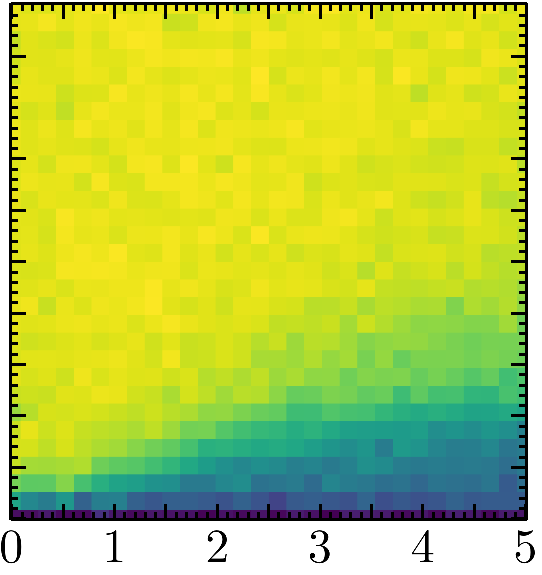
\includegraphics[height=0.333\textwidth]{chaometer_purity_xxz_open_L_7_d_3_Jz_1.00_omega_0.00.pdf}};
\node (legendChaometer) at (chaometer.north) [anchor=south, inner sep=-2pt]  {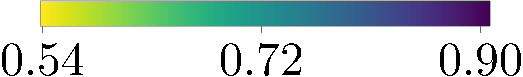
\includegraphics[width=0.27\textwidth]{chaometer_purity_xxz_bar_legend.pdf}};
\node (labelChaometer) at (legendChaometer.north) [anchor=south, inner sep=5pt] {$\overline{\mathcal{P}}$};
\node () at (chaometer.south) [anchor=north, inner sep=-5pt]
 {$\varepsilon/J_z$};
%}

% Averaged Choi purity{
\node (choi) at ([xshift=-6.5pt,yshift=0pt]chaometer.east) [anchor=west] {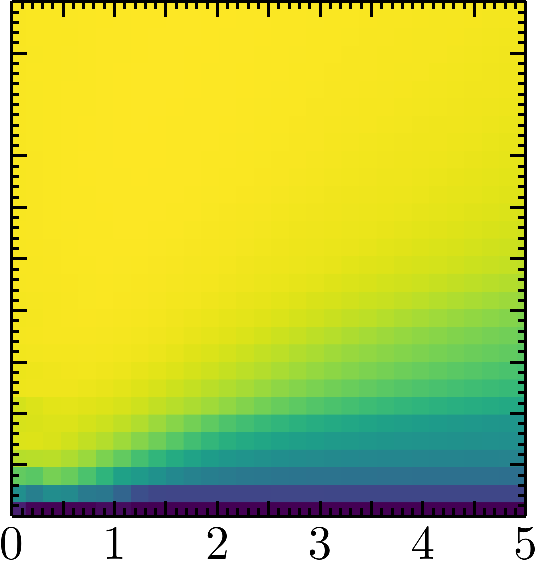
\includegraphics[height=0.333\textwidth]{temporal_avg_haar_avg_choi_purity_xxz_L_7_Jz_1_omega_0_d_3.pdf}};
\node (legendChoi) at (choi.north) [anchor=south, inner sep=-2pt]  {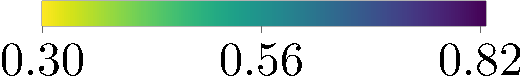
\includegraphics[width=0.27\textwidth]{temporal_avg_haar_avg_choi_purity_xxz_bar_legend.pdf}};
\node (labelchoi) at (legendChoi.north) [anchor=south, inner sep=2pt] {$\ev{\Tr[\mcD(t)^2]}_{\mathrm{Haar}, T}$};
\node () at (choi.south) [anchor=north, inner sep=-5pt] {$\varepsilon/J_z$};
%}

% Letters{
\node (a) at ([xshift=-1.65cm, yshift=0.1cm]labelr.west) {(a)};
\node (b) at ([xshift=3.85cm, yshift=0pt]a.east) {(b)};
\node (c) at ([xshift=3.5cm, yshift=0pt]b.east) {(c)};
%}
\end{scope}
\end{tikzpicture}
\end{document}